\documentclass[letterpaper,12pt]{article}
\usepackage{fullpage}
\usepackage{courier}
\usepackage[margin=0.75in]{geometry}
\usepackage{listings}
\usepackage{color}
\usepackage{graphicx}
\usepackage[width=6in]{caption}
\usepackage{hyphenat}

% define extra colors
\definecolor{dkgreen}{rgb}{0,0.6,0}
\definecolor{purple}{RGB}{159,0,197}

\newcommand*\unparagraph{%
	\par
	\nopagebreak
	\vskip3.25ex plus1ex minus.2ex
	\noindent
}

\lstset{
	language=C++,
	basicstyle=\ttfamily,
	backgroundcolor=\color{white},
	showspaces=false,
	showstringspaces=false,
	frame=none,
	tabsize=3,
	keywordstyle=\color{purple},
	commentstyle=\color{dkgreen},
	stringstyle=\color{blue},
	escapeinside={\%*}{*)}
}

\title{\Large CS 1428\\Quiz 2 Sections L01 and L06} 
\author{Jared Wallace}
\date{}

\begin{document}

\maketitle

\section*{Questions}
\begin{enumerate}
	\item List all of the LOGICAL operators:
		\vspace{20mm}
	\item List all of the RELATIONAL operators:
		\vspace{20mm}
	\item Write a single expression that tests that the variable $grade$ is valid. (i.e. not less than zero or more than 100)
		\vspace{15mm}
	\item What would the result of this expression be?\\
		\lstinline$((4 >= 4 && 8 < 1) || (44 == 33 || 5 > 3))$
		\begin{enumerate}
			\item true
			\item false
		\end{enumerate}

	\newpage

	\item What would the output of this code segment be?
		\lstinputlisting[language=C++]{quizsnippet.cpp}
		\begin{enumerate}
			\item 2
			\item 4
			\item 7
			\item 12
		\end{enumerate}
\end{enumerate}

\vspace{20mm}

\begin{figure}[ht!]
	\centering
	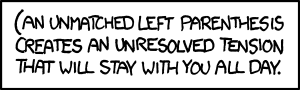
\includegraphics[width=3in]{(.png}
	\caption*{Brains aside, I wonder how many poorly-written xkcd.com-parsing scripts will break on this title$($or ;;``\,`'\{$<<$$[$'this mouseover text''}
\end{figure}

\end{document}
